\documentclass{article}
% Source PDF: :contentReference[oaicite:0]{index=0}

\usepackage{amsmath}
\usepackage{amssymb}
\usepackage{graphicx}
\usepackage{tikz}
\usepackage{pgfplots}
\pgfplotsset{compat=1.18}
\usepackage{booktabs}
\usepackage{xcolor}

\newenvironment{lesson-meta}{}{}        % lesson code, title, objective, EQ, vocab
\newenvironment{item-analysis}{}{}      % Savvas's Example × DOK table
\newenvironment{model-discuss}{}{}      % Launch opener
\newenvironment{concept-box}{}{}        % in-lesson concept reference
\newenvironment{concept-summary}{}{}    % end-of-lesson summary
\newenvironment{example}[1]{}{}         % #1 = example number
\newenvironment{tryit}[1]{}{}           % #1 = tryit number
\newenvironment{practice}[2]{}{}        % #1 = practice number, #2 = DOK
\newenvironment{te-addendum}[2]{}{}     % #1 = anchor example, #2 = type
\newcommand{\answer}[1]{}               % answer key, inside any env
\newcommand{\placeholder}[2]{}          % #1 = type, #2 = description
\newcommand{\uncertain}[2]{#1}          % #1 = best guess, #2 = alternatives
\newcommand{\te}[1]{}                   % teacher-only inline annotation

\begin{document}

\begin{lesson-meta}
Lesson Code: 4-3

Title: Multiplying and Dividing Rational Expressions

I CAN: I can find the product and the quotient of rational expressions.

Objective: Students will be able to use the structure of rational expressions to rewrite simple rational expressions in different forms and understand that rational expressions form a system analogous to the system of rational numbers and use that understanding to multiply and divide rational expressions.

Essential Question: How does multiplying and dividing fractions help you multiply and divide rational expressions?

Essential Understanding: Rational expressions form a system similar to the system of rational numbers and can be multiplied and divided by applying the properties of operations as they apply to rational expressions.

Lesson Vocabulary: simplified form of a rational expression.

Topic Vocabulary: greatest common factor; rational number; rational expression.
\end{lesson-meta}

\begin{item-analysis}
\begin{tabular}{lll}
\toprule
Example & Items & DOK \\
\midrule
1 & 20, 21, 38 & 1 \\
1 & 11, 14--16, 19 & 2 \\
2 & 22--25, 39 & 1 \\
2 & 17, 38 & 2 \\
3 & 26, 27 & 1 \\
3 & 12, 18 & 2 \\
4 & 28, 29 & 1 \\
5 & 30--33 & 1 \\
5 & 40 & 2 \\
5 & 13 & 3 \\
6 & 34, 35 & 1 \\
6 & 36, 37 & 2 \\
\bottomrule
\end{tabular}
\end{item-analysis}

\begin{model-discuss}
Explore \& Reason

Consider the following graph of the function $y=x+2$.

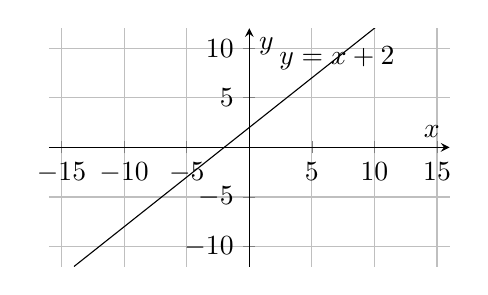
\begin{tikzpicture}
\begin{axis}[
axis lines=middle,
xlabel={$x$},
ylabel={$y$},
xmin=-16,xmax=16,
ymin=-12,ymax=12,
xtick={-15,-10,-5,0,5,10,15},
ytick={-10,-5,0,5,10},
grid=both,
width=0.55\textwidth,
height=0.38\textwidth
]
\addplot[domain=-14:12,samples=2] {x+2};
\node at (axis cs:7,9) {$y=x+2$};
\end{axis}
\end{tikzpicture}

A. What is the domain of this function?

\answer{all real numbers}

B. Sketch a function that resembles the graph, but restrict its domain to exclude 2.

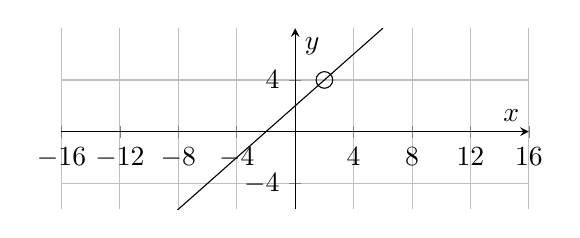
\begin{tikzpicture}
\begin{axis}[
axis lines=middle,
xlabel={$x$},
ylabel={$y$},
xmin=-16,xmax=16,
ymin=-6,ymax=8,
xtick={-16,-12,-8,-4,0,4,8,12,16},
ytick={-4,0,4},
grid=both,
width=0.62\textwidth,
height=0.32\textwidth
]
\addplot[domain=-10:6,samples=2] {x+2};
\addplot[only marks,mark=o,mark size=3pt] coordinates {(2,4)};
\end{axis}
\end{tikzpicture}

\answer{A graph resembling $y=x+2$ with an open circle at $(2,4)$.}

C. Use Structure Consider the function you have sketched. What kind of function might have a graph like this? Explain.

\answer{An equation where the denominator equals zero when $x=2$. For example, $y=\frac{2x-4}{x-2}$.}
\end{model-discuss}

\begin{te-addendum}{ExploreReason}{PurposefulQuestions}
Before --- Implement Tasks that Promote Reasoning and Problem Solving

Q: What do you notice about the graph of the function?
\answer{Sample: $x$-intercept $=-2$; $y$-intercept $=2$; The function is linear.}

During --- Support Productive Struggle in Learning Mathematics

Q: Why is it important to know the domain of a function?
\answer{The domain needs to make sense for the scenario. For example, a real-world problem involving time should remain in Quadrant I on a graph because all numbers should be positive. Also, some values of $x$ cause the function to be undefined, so they cannot be included in the domain.}

For Early Finishers

Q: Sketch the function $y=-x+4$. What is the domain of the function?
\answer{all real numbers}

Q: Sketch the graph of the function, excluding $-4$ from the domain. Describe the new graph created.
\answer{The graph is a linear function with a negative slope and an opening at $x=-4$. The $x$-intercept is 4, and the $y$-intercept is 4.}

After --- Facilitate Meaningful Mathematical Discourse

Discuss the difference between functions that have asymptotes and functions that have discontinuities.

Q: How does the exclusion of an $x$-value in a function's domain due to an asymptote compare to the exclusion of an $x$-value in a function's domain at a single point?
\answer{An asymptote occurs when there is an expression in a fraction's denominator that equals zero and the numerator is not equal to zero for that value. The graph curves on either side of the asymptote and gets close to but never touches it. When the exclusion is at a single point, the graph appears to have a ``hole'' at the excluded value, with the function attaining values ``close'' to the hole.}
\end{te-addendum}

\begin{te-addendum}{ExploreReason}{HabitsOfMind}
Reason Does the graph of $y=\frac{2x+6}{x+3}$ have a vertical asymptote at $x=-3$? Explain.
\answer{No; because the function approaches the point $(-3,2)$ from both sides, there is a hole at $x=-3$ instead of an asymptote.}
\end{te-addendum}

\begin{te-addendum}{1}{LearnTogether}
Introduce students to rational expressions. Explain that multiplying and dividing rational expressions is similar to multiplying and dividing rational numbers.
\end{te-addendum}

\begin{concept-box}
Study Tip

You can make equivalent fractions by multiplying or dividing by a form of 1.
\[
\frac45=\frac45\cdot1=\frac45\cdot\frac22=\frac{8}{10}
\]
\end{concept-box}

\begin{concept-box}
Communicate Precisely

A statement of equivalence between two expressions is an identity. The identity is only valid where both expressions are defined.
\end{concept-box}

\begin{example}{1}
Write Equivalent Rational Expressions

Write an expression that is equivalent to $\frac{x+3}{x+9}$. For what domain are the expressions equivalent?

You can multiply by factors of 1 in any form to write equivalent rational expressions. In this Example, multiply by $\frac{x-6}{x-6}$ and $\frac{x}{x}$.
\[
\frac{x+3}{x+9}
=
\frac{x+3}{x+9}\cdot1\cdot1
\]
\[
=
\frac{x+3}{x+9}\cdot\frac{x-6}{x-6}\cdot\frac{x}{x}
\]
\[
=
\frac{(x+3)(x-6)x}{(x+9)(x-6)x}
\]
\[
=
\frac{x^3-3x^2-18x}{x^3+3x^2-54x}
\]

Since the denominator $x^3+3x^2-54x=x(x+9)(x-6)$, the expression is undefined for $0$, $-9$, and $6$. So the domain must exclude $0$, $-9$, and $6$.

Expressions are equivalent for all values of $x$ that are in both domains. Therefore, $\frac{x+3}{x+9}$ is equivalent to $\frac{x^3-3x^2-18x}{x^3+3x^2-54x}$ over the domain $\{x\mid \text{all real numbers where }x\neq0,6,\text{ or }-9\}$.

\answer{$\frac{x^3-3x^2-18x}{x^3+3x^2-54x}$ over the domain $\{x\mid x\neq0,6,-9\}$.}
\end{example}

\begin{tryit}{1}
Write an expression equivalent to $\frac{x-4}{x}$ over the domain $\{x\mid x\neq0\text{ or }-2\}$.

\answer{$\frac{x^2-2x-8}{x^2+2x}$}
\end{tryit}

\begin{te-addendum}{1}{PurposefulQuestions}
Use and Connect Mathematical Representations

Q: Why is the domain for the identity different from the domain of just the original rational expression?
\answer{Because the equivalence of two expressions must occur where the expressions are both defined.}

Q: Why does the denominator affect the domain but the numerator does not?
\answer{For real values of $x$, a rational expression is the quotient of real numbers. Quotients of real numbers are undefined only when the denominator is 0, and does not depend on the numerator.}

Q: How else can you write an expression equivalent to the original rational expression?
\answer{Multiplying by any other rational expression, such as $\frac{x}{x}$, $\frac{2x}{2x}$, etc., will result in an equivalent rational expression to the original.}
\end{te-addendum}

\begin{te-addendum}{1}{ElicitEvidence}
Q: What are the common factors that occur in both the numerator and the denominator?
\answer{$x+2$}
\end{te-addendum}

\begin{te-addendum}{1}{CommonError}
Try It! 1 Students may think that a common factor $(x-2)$ results in excluding $-2$ from the domain. Have students find the expression or factor when $x=2$. Then ask them for another factor that could result in excluding $-2$ from the domain.
\end{te-addendum}

\begin{te-addendum}{1}{PurposefulQuestions}
Example 1 Have students practice identifying mistakes and determining whether rational expressions are equivalent.

Q: Why are 0 and $-4$ excluded from the domain of the first expression?
\answer{These values make the denominator $4x^4+16x^3=0$, and the denominator cannot equal 0.}

Q: Why is 0 excluded from the domain of the second expression?
\answer{This value makes the denominator $4x^3=0$, and the denominator cannot equal 0.}
\end{te-addendum}

\begin{concept-box}
Common Error

You may not recognize a common factor. Notice that $2-x=-1(-2+x)=-1(x-2)$.
\end{concept-box}

\begin{example}{2}
Simplify a Rational Expression

What is the simplified form of the rational expression? What is the domain for which the identity between the two expressions is valid?
\[
\frac{4-x^2}{x^2+3x-10}
\]

The simplified form of a rational expression has no common factors, other than 1, in the numerator and the denominator.
\[
\frac{4-x^2}{x^2+3x-10}
=
\frac{(2-x)(2+x)}{(x-2)(x+5)}
\]
Factor each polynomial in the numerator and denominator. The domain is all real numbers except 2 and $-5$.
\[
=
\frac{-(x-2)(x+2)}{(x-2)(x+5)}
\]
Common factors divide to 1, so
\[
\frac{-(x-2)(x+2)}{(x-2)(x+5)}
=
-\frac{(x-2)}{(x-2)}\cdot\frac{x+2}{x+5}
=
-1\cdot\frac{x+2}{x+5}.
\]

The simplified form of $\frac{4-x^2}{x^2+3x-10}$ is $-\frac{x+2}{x+5}$ for $x\neq2$ or $-5$.

\answer{$-\frac{x+2}{x+5}$ for $x\neq2,-5$.}
\end{example}

\begin{tryit}{2}
Simplify each expression and state the domain.

a. $\frac{x^2+2x+1}{x^3-2x^2-3x}$

b. $\frac{x^3+4x^2-x-4}{x^2+3x-4}$

\answer{a. $\frac{x+1}{x(x-3)}$ for all $x$ except $0$, $-1$, and $3$. b. $x+1$ for all $x$ except $1$ and $-4$.}
\end{tryit}

\begin{te-addendum}{2}{PurposefulQuestions}
Pose Purposeful Questions

Q: Why is $-1$ factored out of $2-x$ in the numerator?
\answer{If you factor out $-1$, you can divide out the common factor $x-2$.}

Q: Why can you cross out factors that divide to 1?
\answer{A rational expression with factors that divide to 1 can be written as 1 times another rational expression, and 1 is not typically written in products.}
\end{te-addendum}

\begin{concept-box}
Use Structure

Notice that the product of rational expressions is a rational expression. How can you use the definition of rational expressions to show that rational expressions are closed under multiplication?
\end{concept-box}

\begin{example}{3}
Multiply Rational Expressions

A. What is the product of $\frac{2xy}{z}$ and $\frac{3x^2}{4yz}$?

To multiply rational expressions, follow a similar method to that for multiplying two numerical fractions.
\[
\frac{2xy}{z}\cdot\frac{3x^2}{4yz}
=
\frac{(2xy)(3x^2)}{z(4yz)}
\]
\[
=
\frac{2\cdot3\cdot y\cdot x^3}{2\cdot2\cdot y\cdot z^2}
\]
\[
=
\frac{3x^3}{2z^2}
\]
The product of $\frac{2xy}{z}$ and $\frac{3x^2}{4yz}$ is $\frac{3x^3}{2z^2}$ for $y\neq0$ and $z\neq0$.

B. What is the product of $\frac{5x}{x+3}\cdot\frac{x^2+x-6}{x^2+2x+1}\cdot\frac{x^2+x}{5x-10}$ in simplified form?
\[
\frac{5x}{x+3}\cdot\frac{x^2+x-6}{x^2+2x+1}\cdot\frac{x^2+x}{5x-10}
=
\frac{5x(x+3)(x-2)x(x+1)}{(x+3)(x+1)(x+1)5(x-2)}
\]
\[
=
\frac{5x^2(x+3)(x-2)(x+1)}{5(x+3)(x-2)(x+1)(x+1)}
\]
\[
=
\frac{x^2}{x+1}
\]
So,
\[
\frac{5x}{x+3}\cdot\frac{x^2+x-6}{x^2+2x+1}\cdot\frac{x^2+x}{5x-10}
=
\frac{x^2}{x+1}
\]
for $x\neq-3,-1,$ or $2$.

\answer{A. $\frac{3x^3}{2z^2}$ for $y\neq0$ and $z\neq0$. B. $\frac{x^2}{x+1}$ for $x\neq-3,-1,2$.}
\end{example}

\begin{tryit}{3}
Find the simplified form of each product, and state the domain.

a. $\frac{x^2-16}{9-x}\cdot\frac{x^2+x-90}{x^2+14x+40}$

b. $\frac{x+3}{4x}\cdot\frac{3x-18}{6x+18}\cdot\frac{x^2}{4x+12}$

\answer{a. $-(x-4)$ for all $x$ except $9$, $-10$, and $-4$. b. $\frac{x(x-6)}{32(x+3)}$ for all $x$ except $0$ and $-3$.}
\end{tryit}

\begin{te-addendum}{3}{PurposefulQuestions}
Pose Purposeful Questions

Part A

Q: How can you determine that the domain is $z\neq0$ and $y\neq0$ by looking at the rational expressions?
\answer{The denominator cannot equal 0 because the rational expression would be undefined. Therefore, $z\neq0$ and $y\neq0$ because multiplying 0 by any number is 0.}

Part B

Q: Why do you factor the expressions in the numerator and the denominator?
\answer{You can divide out the common factors, and you can determine the restrictions on the domain by using the Zero Product Property.}
\end{te-addendum}

\begin{te-addendum}{1}{HabitsOfMind}
Use with Examples 1 \& 2

Critique Reasoning Bailey simplified the rational expression $\frac{x^2+2x+4}{x^2+x+2}$ by dividing out the $x^2$-terms and then dividing out a factor of $x+2$ to get 2 as the simplified form of the rational expression. Is Bailey correct? Why or why not?
\answer{No; you cannot eliminate terms from the numerator and denominator if they are bound by addition. You must factor the expression first, and then eliminate like factors.}
\end{te-addendum}

\begin{te-addendum}{3}{RtIExtend}
Use with Example 3 Challenge students to write an expression as the product of two rational expressions with the given domain.

Q: The domain of the product of two rational expressions is all real numbers except $0$, $-3$, and $6$.
\answer{Sample: $\frac{1}{x^2+3x}\cdot\frac{1}{x-6}$.}
\end{te-addendum}

\begin{te-addendum}{4}{PurposefulQuestions}
Example 4 Help students transition to multiplying more than one rational expression by a polynomial.

Q: How does multiplying two rational expressions and a polynomial compare with multiplying two rational expressions or a rational expression and a polynomial?
\answer{They are all like multiplying fractions. The polynomials are written as rational expressions with a denominator of 1.}
\end{te-addendum}

\begin{concept-box}
Common Error

Only common factors, not terms, reduce to one. You cannot factor an $x$ out of $\frac{x}{x^2+4}$.
\end{concept-box}

\begin{example}{4}
Multiply a Rational Expression by a Polynomial

What is the product of $\frac{x+2}{x^4-16}$ and $x^3+4x^2-12x$?
\[
\frac{x+2}{x^4-16}\cdot(x^3+4x^2-12x)
=
\frac{x+2}{x^4-16}\cdot\frac{x^3+4x^2-12x}{1}
\]
Write 1 in the denominator to keep track of positions of factors.
\[
=
\frac{(x+2)x(x^2+4x-12)}{1(x^2+4)(x^2-4)}
\]
\[
=
\frac{(x+2)x(x+6)(x-2)}{1(x^2+4)(x+2)(x-2)}
\]
The domain is $x\neq-2,$ or $2$.
\[
\text{So } \frac{x+2}{x^4-16}\cdot(x^3+4x^2-12x)=\frac{x(x+6)}{x^2+4}
\]
for $x\neq-2$ or $2$.

\answer{$\frac{x(x+6)}{x^2+4}$ for $x\neq-2,2$.}
\end{example}

\begin{tryit}{4}
Find the simplified form of each product and the domain.

a. $\frac{x^3-4x}{6x^2-13x-5}\cdot(2x^3-3x^2-5x)$

b. $\frac{3x^2+6x}{x^2-49}\cdot(x^2+9x+14)$

\answer{a. $\frac{x^2(x+2)(x-2)(x+1)}{3x+1}$ for all $x$ except $\frac52$ and $-\frac13$. b. $\frac{3x(x+2)^2}{x-7}$ for all $x$ except $7$ and $-7$.}
\end{tryit}

\begin{te-addendum}{4}{PurposefulQuestions}
Use and Connect Mathematical Representations

Q: What do you already know about multiplying a fraction and a whole number that is helpful here?
\answer{To multiply a fraction and a whole number, you need to also make the whole number a fraction with a denominator of 1.}

Q: Is there a number for $x$ that would make $x^2+4=0$?
\answer{No; squaring any number, whether negative or positive, results in a positive number. Adding two positive numbers will never equal 0.}
\end{te-addendum}

\begin{te-addendum}{3}{HabitsOfMind}
Use with Examples 3 \& 4

Generalize Why is it important to identify the domain of a rational expression before you simplify it rather than after?
\answer{Simplifying the expression may eliminate some values where the original expression is undefined.}
\end{te-addendum}

\begin{concept-box}
Use Structure

This division problem could be written as a complex fraction.
\[
\frac{\frac{x^3+3x^2+3x+1}{1-x^2}}{\frac{x^2+5x+4}{x^2+3x-4}}
\]
You can rewrite any complex fraction as a division statement.
\end{concept-box}

\begin{example}{5}
Divide Rational Expressions

What is the quotient of $\frac{x^3+3x^2+3x+1}{1-x^2}$ and $\frac{x^2+5x+4}{x^2+3x-4}$?
\[
\frac{x^3+3x^2+3x+1}{1-x^2}
\div
\frac{x^2+5x+4}{x^2+3x-4}
=
\frac{x^3+3x^2+3x+1}{1-x^2}
\cdot
\frac{x^2+3x-4}{x^2+5x+4}
\]
Multiply by the reciprocal of the divisor.
\[
=
\frac{(x+1)(x+1)(x+1)(x+4)(x-1)}{-(x-1)(x+1)(x+1)(x+4)}
\]
The domain is $x\neq-4,-1,$ or $1$.
\[
=
\frac{x+1}{-1}\cdot
\frac{x+1}{x+1}\cdot
\frac{x+1}{x+1}\cdot
\frac{x-1}{x-1}\cdot
\frac{x+4}{x+4}
\]
\[
=-(x+1)
\]
The quotient is $-(x+1)$, $x\neq-4,-1,$ or $1$.

\answer{$-(x+1)$ for $x\neq-4,-1,1$.}
\end{example}

\begin{tryit}{5}
Find the simplified quotient and the domain of each expression.

a. $\frac{1}{x^2+9x}\div\left(\frac{6-x}{3x^2-18x}\right)$

b. $\frac{2x^2-12x}{x+5}\div\left(\frac{x-6}{x+5}\right)$

\answer{a. $-\frac{3}{x+9}$ for all $x$ except $0$, $-9$, and $6$. b. $2x$ for all $x$ except $6$ and $-5$.}
\end{tryit}

\begin{te-addendum}{5}{PurposefulQuestions}
Pose Purposeful Questions

Q: Why do you factor out $-1$?
\answer{The factoring out of $-1$ allows you to divide common factors from the numerator and the denominator.}

Q: How is dividing rational expressions similar to dividing fractions?
\answer{You multiply by the reciprocal of the divisor.}
\end{te-addendum}

\begin{te-addendum}{5}{RtISupport}
Use with Example 5 Students have the opportunity for guided practice in dividing two rational expressions.

Divide
\[
\frac{3x^3+6x^2+3x}{x+2}\div\frac{x^2+x}{x+2}.
\]
Multiply by the reciprocal of the divisor. Factor the numerators and denominators individually. Divide out the common factors.

Q: How do you decide what can be factored out of each expression?
\answer{Find the greatest common factor.}

Q: What are the quotient and the domain?
\answer{$3(x+1)$; $x\neq-2,-1,0$}
\end{te-addendum}

\begin{concept-box}
Study Tip

Recall that surface area tells how much packaging material is needed and volume tells how much product the packaging can hold.
\end{concept-box}

\begin{example}{6}
Use Division of Rational Expressions

\placeholder{illustration}{Two package designs: a rectangular box and a cylindrical package.}

A company is evaluating two packaging options for its product line. The more efficient design will have the lesser ratio of surface area to volume. Should the company use packages that are cylinders or rectangular prisms?

Option 1: A rectangular prism with a square base.

Option 2: A cylinder with the same height as the prism, and diameter equal to the side length of the prism's base.

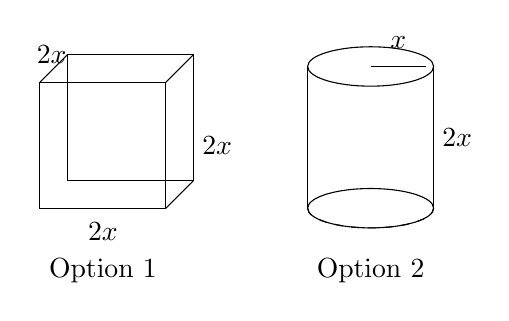
\begin{tikzpicture}
\draw (0,0) rectangle (1.6,1.6);
\draw (0.35,0.35) rectangle (1.95,1.95);
\draw (0,1.6)--(0.35,1.95);
\draw (1.6,1.6)--(1.95,1.95);
\draw (1.6,0)--(1.95,0.35);
\node at (0.8,-0.3) {$2x$};
\node at (2.25,0.8) {$2x$};
\node at (0.15,1.95) {$2x$};
\node at (0.8,-0.8) {Option 1};

\draw (4.2,0) ellipse (0.8 and 0.25);
\draw (3.4,0)--(3.4,1.8);
\draw (5.0,0)--(5.0,1.8);
\draw (4.2,1.8) ellipse (0.8 and 0.25);
\draw[dashed] (3.4,0) arc[start angle=180,end angle=360,x radius=0.8,y radius=0.25];
\draw (4.2,1.8)--(4.9,1.8);
\node at (4.55,2.1) {$x$};
\node at (5.3,0.9) {$2x$};
\node at (4.2,-0.8) {Option 2};
\end{tikzpicture}

Surface Area for Option 1:
\[
2(2x)^2+4(2x)^2
\]
Volume for Option 1:
\[
(2x)^3
\]
Surface Area for Option 2:
\[
2\pi x^2+2\pi x(2x)
\]
Volume for Option 2:
\[
\pi x^2(2x)
\]

The efficiency ratio is $\frac{SA}{V}$, where $SA$ represents surface area and $V$ represents volume.

Option 1:
\[
\frac{SA}{V}
=
\frac{2(4x^2)+4(4x^2)}{8x^3}
=
\frac{24x^2}{8x^3}
=
\frac3x
\]

Option 2:
\[
\frac{SA}{V}
=
\frac{2\pi x^2+4\pi x^2}{2\pi x^3}
=
\frac{6\pi x^2}{2\pi x^3}
=
\frac3x
\]

The company can now compare the efficiency ratio of the package designs.

Prism: $\frac3x$

Cylinder: $\frac3x$

In this example, the efficiency ratio of the cylinder is equal to that of the prism. So the company should choose their package design based on other criteria.

\begin{concept-box}
Regardless of what positive value is selected for $x$, the efficiency ratios for these two package designs will be the same.
\end{concept-box}

\answer{The prism and cylinder both have efficiency ratio $\frac3x$; the company should choose the package design based on other criteria.}
\end{example}

\begin{tryit}{6}
The company compares the ratios of surface area to volume for two more containers. One is a rectangular prism with a square base. The other is a rectangular prism with a rectangular base. One side of the base is equal to the side length of the first container, and the other side is twice as long. The surface area of this second container is $4x^2+6xh$. The heights of the two containers are equal. Which has the smaller surface area-to-volume ratio?

\answer{The efficiency ratio for the prism with the rectangular base is less than that for the prism with the square base.}
\end{tryit}

\begin{te-addendum}{6}{PurposefulQuestions}
Pose Purposeful Questions

Q: What does it mean to have the lesser ratio of surface area to volume?
\answer{the division of surface area by volume that results in a smaller rational expression}

Q: How do the efficiency ratios of the rectangular prism and the cylinder compare to each other?
\answer{The rectangular prisms and the cylinder will always have the same efficiency ratio, regardless of the $x$-value selected.}
\end{te-addendum}

\begin{te-addendum}{5}{HabitsOfMind}
Use with Examples 5 \& 6

Use Structure Is the domain of the quotient
\[
\frac{2x^2-12x}{x+5}\div\left(\frac{x-6}{x+5}\right)
\]
different from the domain of the product
\[
\left(\frac{2x^2-12x}{x+5}\right)\left(\frac{x-6}{x+5}\right)?
\]
Explain.
\answer{Yes; the domain of the product includes the value $x=6$, while the domain of the quotient does not include $x=6$.}
\end{te-addendum}

\begin{te-addendum}{6}{ELLAddendum}
English Language Learners

Speaking --- Beginning

When you evaluate something, you assign it a value or level of importance. Display a pen, a stapler, a paper clip, and a cell phone. Have students discuss the following questions in small groups.

Q: How would you arrange these items from lowest to highest in value?
\answer{paper clip, pen, stapler, cell phone}

Q: Why would the packaging with a lesser ratio of surface area to volume be more valuable to a company?
\answer{If the company spends less on packaging, they can make a larger profit.}

Reading --- Developing

Have students read the problem statement in the example. Have students point to the words ratio, surface area, and volume as they read them.

Q: What does surface area mean?
\answer{the sum of the areas of all of the outside surfaces of an object}

Q: What does volume mean?
\answer{the capacity an object can hold, or the amount of space it takes up}

Q: Why is the design with the lesser ratio of surface area to volume more efficient?
\answer{because the packaging would use less material to contain a given volume}

Listening --- Expanding

Distribute a piece of construction paper and a pair of scissors to pairs of students. Ask students to cut the paper into 5 or 6 polygons and mix them up. Have one person put the puzzle pieces back together while the other records the time it takes. Then switch roles. Have students repeat this exercise with their eyes closed. Listen to the definition of efficient: ``performing in the best possible manner with the least waste of time and effort.''

Q: Which method of putting the puzzle together was more efficient? Explain.
\answer{The first method was more efficient.}
\end{te-addendum}

\begin{concept-summary}
Products and Quotients of Rational Expressions

\begin{tabular}{llll}
\toprule
 & Multiply & Multiply an Integer or a Polynomial & Divide \\
\midrule
Rational Expressions &
$\frac{3x}{x+1}\cdot\frac{x^2+x}{3x-6}$ &
$\frac{x+2}{x^2-4}\cdot(x^2-2x)$ &
$\frac{1-x^2}{x^2+3x-4}\div\frac{x+1}{x+4}$ \\
Domain &
$x\neq-1$ or $2$ &
$x\neq-2$ or $2$ &
$x\neq-4,-1,$ or $1$ \\
Words &
Identify common factors and simplify. &
Write the polynomial as a rational expression with 1 in the denominator. Then multiply. &
Multiply by the reciprocal of the divisor. \\
\bottomrule
\end{tabular}

Do You UNDERSTAND?

1. Essential Question How does multiplying and dividing fractions help you multiply and divide rational expressions?
\answer{The steps and operations used to multiply and divide rational expressions are similar to those used with fractions.}

2. Vocabulary In your own words, define rational expression and provide an example of a rational expression.
\answer{A rational expression is the ratio of two polynomials that has a domain of all real numbers except those for which the denominator equals zero; Sample: $\frac{3x^2+6x}{9x}$.}

3. Error Analysis A student divided the rational expressions as follows:
\[
\frac{4x}{5y}\div\frac{20x^2}{25y^2}
=
\frac{4x}{5y}\div\frac{5\cdot4x^2}{25y^2}
=
\frac{16x^3}{25y^3}.
\]
Describe and correct the errors the student made.
\answer{The student was supposed to multiply by the reciprocal. The student also did not place any restrictions on the domain. The rational expression should be $\frac{y}{x}$, $x\neq0$, $y\neq0$.}

4. Communicate Precisely Why do you have to state the domain when simplifying rational expressions?
\answer{When the denominator equals 0, fractions are undefined.}

Do You KNOW HOW?

5. What is the simplified form of the rational expression $\frac{x^2-36}{x^2+3x-18}$? What is the domain?
\answer{$\frac{x-6}{x-3}$ for all $x$ except $-6$ and $3$.}

Find the simplified form of each product, and state the domain.

6. $\frac{4x^2y^2}{3z}\cdot\frac{15z^2}{20xy^3}$
\answer{$\frac{xz}{y}$, $x\neq0$, $y\neq0$, and $z\neq0$.}

7. $\frac{y+3}{y+2}\cdot\frac{y^2+4y+4}{y^2-9}$
\answer{$\frac{y+2}{y-3}$, $y\neq-3$, $3$, or $-2$.}

8. $\frac{x^2+3x-10}{x^2-25}\cdot(x^2-9x+20)$
\answer{$(x-2)(x-4)$ for all $x$ except $5$ and $-5$.}

Find the simplified form of each quotient, and state the domain.

9. $\frac{x^3+14x^2+49x}{x^2+3x-28}\div(x+7)$
\answer{$\frac{x}{x-4}$ for all $x$ except $4$ and $-7$.}

10. $\frac{6x^4+21x^3-12x^2}{x^3+x^2-36x-36}\div\frac{12x^2-6x}{4x^2-144}$
\answer{$\frac{2x(x+4)}{x+1}$ for all $x$ except $-6$, $6$, $-1$, $0$, and $\frac12$.}
\end{concept-summary}

\begin{te-addendum}{ConceptSummary}{PurposefulQuestions}
Q: How do multiplying or dividing rational expressions compare to multiplying or dividing fractions?
\answer{When multiplying rational expressions and multiplying fractions, you write a whole number and the expression with a denominator of 1 and then identify common factors and simplify. When dividing rational expressions and dividing fractions, you multiply by the reciprocal of the divisor.}
\end{te-addendum}

\begin{te-addendum}{5}{CommonError}
Exercise 9 Students may struggle with division when the divisor is a polynomial instead of a rational expression. Ask students how the polynomial can be written as a rational expression. Then ask students how they can write the quotient of rational expressions as a product of rational expressions.
\end{te-addendum}

\begin{practice}{11}{2}
Reason Explain why $\frac{4x^2-7}{4x^2-7}=1$ is a valid identity under the domain of all real numbers except $\pm\frac{\sqrt7}{2}$.

\answer{Using the difference of two squares formula, $\frac{4x^2-7}{4x^2-7}=\frac{(2x+\sqrt7)(2x-\sqrt7)}{(2x+\sqrt7)(2x-\sqrt7)}$. Both factors on the numerator and denominator divide to 1, so $\frac{4x^2-7}{4x^2-7}=1$ over all elements of the domain, which is all real numbers except $\pm\frac{\sqrt7}{2}$.}
\end{practice}

\begin{practice}{12}{2}
Error Analysis Describe the error a student made in multiplying and simplifying
\[
\frac{x+2}{x-2}\cdot\frac{x^2-4}{x^2+x-2}.
\]
Student work:
\[
\frac{x+2}{x-2}\cdot\frac{x^2-4}{x^2+x-2}
=
\frac{x+2}{x-2}\cdot\frac{(x+2)(x-2)}{(x+2)(x-1)}
=
\frac{2}{-1}.
\]

\answer{The student cannot cancel the $x$'s in $x+2$ and $x-1$ because only common factors, not terms, can be canceled.}
\end{practice}

\begin{practice}{13}{3}
Higher Order Thinking Why are rational expressions closed under multiplication and division?

\answer{Sample: $\frac{a}{b}\div\frac{c}{d}=\frac{\frac{a}{b}}{\frac{c}{d}}=\frac{\frac{a}{b}}{\frac{c}{d}}\times\frac{\frac{d}{c}}{\frac{d}{c}}=\frac{ad}{bc}\div\frac{cd}{dc}=\frac{ad}{bc}\div1=\frac{ad}{bc}=\frac{a}{b}\times\frac{d}{c}$.}
\end{practice}

\begin{practice}{14}{2}
Use Appropriate Tools Explain why domain restrictions are necessary to show that the rational expressions $\frac{-6x^2+21x}{3x}$ and $-2x+7$ are equivalent. What is true about the graphs at $x=0$ and why?

\answer{Sample answer: Domain restrictions are needed because you may not be able to tell just from graphs when two expressions are not equivalent. The graphs of $y=\frac{-6x^2+21x}{3x}$ and $y=-2x+7$ may look identical, but using the trace feature or a table values, $y=\frac{-6x^2+21x}{3x}$ is undefined at $x=0$, while $y=-2x+7$ is equal to 7 at $x=0$.}
\end{practice}

\begin{practice}{15}{2}
Generalize Explain the similarities between rational numbers and rational expressions.

\answer{A rational number is the ratio of two integers, while a rational expression is a ratio of two polynomials.}
\end{practice}

\begin{practice}{16}{2}
Use Structure Determine whether $\frac{5x+11}{6x+11}=\frac56$ is sometimes, always, or never true. Justify your reasoning.

\answer{Never; when you cross multiply, you get $30x+66=30x+55$; since $66\neq55$, there is no real number $x$ for which that equation is true.}
\end{practice}

\begin{practice}{17}{2}
Construct Arguments Explain how you can tell whether a rational expression is in simplest form.

\answer{A rational expression is in simplest form when the numerator and denominator have no common factors other than 1.}
\end{practice}

\begin{practice}{18}{2}
Communicate Precisely When multiplying $\frac{15}{x}\cdot\frac{x}{3}=5$, is it necessary to make the restriction $x\neq0$? Why or why not?

\answer{Yes; even though the factor of $x$ was canceled out, the original fractions cannot be undefined, so the restriction is necessary.}
\end{practice}

\begin{practice}{19}{2}
Reason If the denominator of a rational expression is $x^3+3x^2-10x$, what value(s) must be restricted from the domain for $x$?

\answer{$-5$, $0$, $2$}
\end{practice}

\begin{practice}{20}{1}
Write an equivalent expression over the given domain.

\[
\frac{x(x-2)}{x-5}
\]
for all $x$ except $5$ and $-6$.

\answer{$\frac{x^3+4x^2-12x}{x^2+x-30}$}
\end{practice}

\begin{practice}{21}{1}
Write an equivalent expression over the given domain.

\[
\frac{3x}{x-2}
\]
for all $x$ except $2$ and $-5$.

\answer{$\frac{3x^2+15x}{x^2+3x-10}$}
\end{practice}

\begin{practice}{22}{1}
What is the simplified form of the rational expression? What is the domain?
\[
\frac{y^2-5y-24}{y^2+3y}
\]

\answer{$\frac{y-8}{y}$ for all $y$ except $0$ and $-3$.}
\end{practice}

\begin{practice}{23}{1}
What is the simplified form of the rational expression? What is the domain?
\[
\frac{ab^3-9ab}{12ab^2+12ab-144a}
\]

\answer{$\frac{b(b+3)}{12(b+4)}$ for all real numbers except $a=0$, $b=-4$, and $b=3$.}
\end{practice}

\begin{practice}{24}{1}
What is the simplified form of the rational expression? What is the domain?
\[
\frac{x^2+8x+15}{x^2-x-12}
\]

\answer{$\frac{x+5}{x-4}$, $x\neq-3,4$.}
\end{practice}

\begin{practice}{25}{1}
What is the simplified form of the rational expression? What is the domain?
\[
\frac{x^3+9x^2-10x}{x^3-9x^2-10x}
\]

\answer{$\frac{(x+10)(x-1)}{(x-10)(x+1)}$, $x\neq-1,0,10$.}
\end{practice}

\begin{practice}{26}{1}
Find the product and the domain.
\[
\frac{x^2+6x+8}{x^2+4x+3}\cdot\frac{x+3}{x+2}
\]

\answer{$\frac{x+4}{x+1}$ for all $x$ except $-3$, $-2$, and $-1$.}
\end{practice}

\begin{practice}{27}{1}
Find the product and the domain.
\[
\frac{(x-y)^2}{x+y}\cdot\frac{3x+3y}{x^2-y^2}
\]

\answer{$\frac{3(x-y)}{x+y}$ for all real numbers except $x=y$ or $x=-y$.}
\end{practice}

\begin{practice}{28}{1}
Find the product and the domain.
\[
\frac{x+5}{x^3-25x}\cdot(2x^3-11x^2+5x)
\]

\answer{$2x-1$ for all $x$ except $0$, $-5$, and $5$.}
\end{practice}

\begin{practice}{29}{1}
Find the product and the domain.
\[
\frac{2x^2-10x}{(x-5)(x^2-1)}\cdot(3x^2+4x+1)
\]

\answer{$\frac{2x(3x+1)}{x-1}$ for all $x$ except $-1$, $1$, and $5$.}
\end{practice}

\begin{practice}{30}{1}
Find the quotient and the domain.
\[
\frac{y^2-16}{y^2-10y+25}\div\frac{3y-12}{y^2-3y-10}
\]

\answer{$\frac{(y+4)(y+2)}{3(y-5)}$ for all $y$ except $4$ and $5$.}
\end{practice}

\begin{practice}{31}{1}
Find the quotient and the domain.
\[
\frac{(x-y)^2}{x+y}\div\frac{3x+3y}{x^2-y^2}
\]

\answer{$\frac{(x-y)^3}{3(x+y)}$ for all $x$ except $x=-y$.}
\end{practice}

\begin{practice}{32}{1}
Find the quotient and the domain.
\[
\frac{25x^2-4}{x^2-9}\div\frac{5x-2}{x+3}
\]

\answer{$\frac{5x+2}{x-3}$ for all $x$ except $-3$, $\frac25$, and $3$.}
\end{practice}

\begin{practice}{33}{1}
Find the quotient and the domain.
\[
\frac{x^4+x^3-30x^2}{x^2-3x-18}\div\frac{x^3+x^2-30x}{x^2-36}
\]

\answer{$\frac{x(x+6)}{x+3}$, $x\neq-6,-3,0,5,6$.}
\end{practice}

\begin{practice}{34}{1}
Find and simplify the ratio of the volume of Figure A to the volume of Figure B.

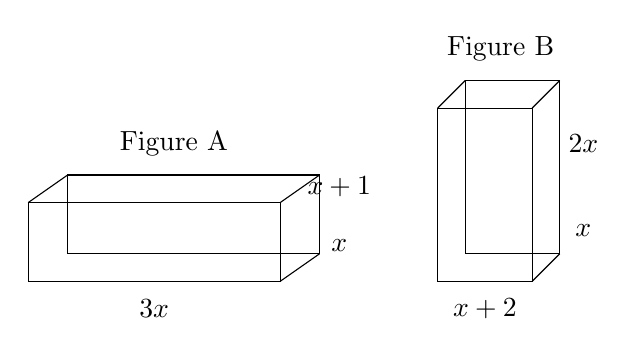
\begin{tikzpicture}
\draw (0,0) rectangle (3.2,1.0);
\draw (0.5,0.35) rectangle (3.7,1.35);
\draw (0,1.0)--(0.5,1.35);
\draw (3.2,1.0)--(3.7,1.35);
\draw (3.2,0)--(3.7,0.35);
\node at (1.6,-0.35) {$3x$};
\node at (3.95,0.45) {$x$};
\node at (3.95,1.2) {$x+1$};
\node at (1.85,1.75) {Figure A};

\draw (5.2,0) rectangle (6.4,2.2);
\draw (5.55,0.35) rectangle (6.75,2.55);
\draw (5.2,2.2)--(5.55,2.55);
\draw (6.4,2.2)--(6.75,2.55);
\draw (6.4,0)--(6.75,0.35);
\node at (5.8,-0.35) {$x+2$};
\node at (7.05,0.65) {$x$};
\node at (7.05,1.75) {$2x$};
\node at (6.0,2.95) {Figure B};
\end{tikzpicture}

\answer{$\frac{3(x+1)}{2(x+2)}$ for all $x>0$.}
\end{practice}

\begin{practice}{35}{1}
Make Sense and Persevere An engineering firm wants to construct a cylindrical structure that will maximize the volume for a given surface area. Compare the ratios of the volume to surface area of each of the cylindrical structures shown, using the following formulas for volume and surface area of cylinders.

Volume $(V)=\pi r^2h$

Surface Area $(SA)=2\pi rh+2\pi r^2$

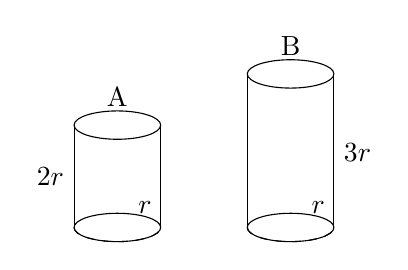
\begin{tikzpicture}
\draw (0,0) ellipse (0.55 and 0.18);
\draw (-0.55,0)--(-0.55,1.3);
\draw (0.55,0)--(0.55,1.3);
\draw (0,1.3) ellipse (0.55 and 0.18);
\draw[dashed] (-0.55,0) arc[start angle=180,end angle=360,x radius=0.55,y radius=0.18];
\node at (-0.85,0.65) {$2r$};
\node at (0.35,0.25) {$r$};
\node at (0,1.65) {A};

\draw (2.2,0) ellipse (0.55 and 0.18);
\draw (1.65,0)--(1.65,1.95);
\draw (2.75,0)--(2.75,1.95);
\draw (2.2,1.95) ellipse (0.55 and 0.18);
\draw[dashed] (1.65,0) arc[start angle=180,end angle=360,x radius=0.55,y radius=0.18];
\node at (3.05,0.95) {$3r$};
\node at (2.55,0.25) {$r$};
\node at (2.2,2.3) {B};
\end{tikzpicture}

a. Calculate the ratio of volume to surface area for cylinder A.

b. Calculate the ratio of volume to surface area for cylinder B.

c. Which of these cylinders has a greater ratio of volume to surface area?

\answer{a. $\frac{r}{3}$ b. $\frac{3r}{8}$ c. cylinder B}
\end{practice}

\begin{practice}{36}{2}
Model With Mathematics Lupe designed a carnival game that involves tossing a beanbag into the box shown. In order to win a prize, the beanbag must fall inside the black rectangle. The probability of winning is equal to the ratio of the area of the black rectangle to the total area of the face of the box shown. Find the ratio that represents this probability in simplified form.

\placeholder{illustration}{Carnival beanbag toss scene with a person tossing a beanbag toward a rectangular game board.}

\begin{tikzpicture}
\draw (0,0) rectangle (5.2,2.2);
\node at (2.6,-0.35) {$3x$};
\node[rotate=90] at (-0.35,1.1) {$x+1$};
\draw (3.0,0.65) rectangle (4.4,1.35);
\node at (3.7,1.65) {$x$};
\node at (2.55,1.0) {$\frac12x$};
\end{tikzpicture}

\answer{The probability is $\frac{x}{6(x+1)}$.}
\end{practice}

\begin{practice}{37}{2}
Look for Relationships A parallelogram with an area of $\frac{3x+12}{10x+25}$ square units has a height shown. Find the length of the base of the parallelogram.

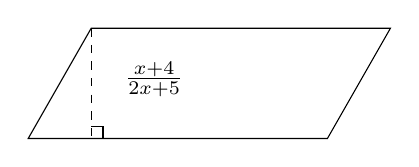
\begin{tikzpicture}
\draw (0,0)--(3.8,0)--(4.6,1.4)--(0.8,1.4)--cycle;
\draw[dashed] (0.8,1.4)--(0.8,0);
\draw (0.8,0.15)--(0.95,0.15)--(0.95,0);
\node at (1.6,0.75) {$\frac{x+4}{2x+5}$};
\end{tikzpicture}

\answer{The length of the base of the parallelogram is $\frac35$ units.}
\end{practice}

\begin{practice}{38}{1/2}
Which of the following rational expressions simplify to $\frac{y}{y+3}$? Select all that apply.

\[
\frac{(2y^2+y)(y+3)}{(4y+2)(y+3)^2}
\]
\[
\frac{3y^2+y}{3y^2+10y+3}
\]
\[
\frac{2y^3+3y^2+y}{(2y+1)(y^2+4y+3)}
\]
\[
\frac{y^2+2y}{y^2+4y+3}
\]
\[
\frac{\frac1y}{y+3}
\]

\answer{$\frac{3y^2+y}{3y^2+10y+3}$ and $\frac{2y^3+3y^2+y}{(2y+1)(y^2+4y+3)}$}
\end{practice}

\begin{practice}{39}{1}
SAT/ACT For what value of $x$ is $\frac{2x^2+8x}{(x+4)(x^2-9)}$ undefined?

A. $-8$

B. $-3$

C. $0$

D. $4$

E. $9$

\answer{B. $-3$}
\end{practice}

\begin{practice}{40}{2}
Performance Task The approximate annual interest rate $r$ of a monthly installment loan is given by the formula:
\[
r=\frac{\left[\frac{24(nm-p)}{n}\right]}{p+\frac{nm}{12}},
\]
where $n$ is the total number of payments, $m$ is the monthly payment, and $p$ is the amount financed.

Part A Find the approximate annual interest rate (to the nearest percent) for a four-year signature loan of $\$20{,}000$ that has monthly payments of $\$500$.

Part B Find the approximate annual interest rate (to the nearest tenth percent) for a five-year auto loan of $\$40{,}000$ that has monthly payments of $\$750$.

\answer{Part A $9\%$; Part B $4.6\%$}
\end{practice}

\end{document}